\documentclass[732,14pt,final]{studrep}

\RequirePackage{tabularx}
% \RequirePackage{graphicx}
% Тестирование изменений
% \usepackage{showframe}

% test 

% pygmetize 
\RequirePackage{minted}
\RequirePackage{indentfirst}
\RequirePackage{graphicx}
\usemintedstyle{tango} % bw
\RequirePackage{doi}

% \setmainfont{Times New Roman}
\graphicspath{{pics/}}


\setminted{autogobble,mathescape,linenos=true,fontsize=\small,breaklines}
\begin{document}
\thispagestyle{empty}
\clearpage
 
\tableofcontents

\chapter*{ВВЕДЕНИЕ}
\label{chap:intro}
% TODO: Add contents line


\subsection*{Автоматизация распознавания береговой линии: обзор технологий}

Фундаментальные исследования уникальных экологических систем, какой является береговая зона крупного водного объекта, проводимые в мире и России, базируются на мониторинге, основывающимся на больших данных. Мониторинг опасных экзогенных геологических процессов входит в единую информационную систему Государственного мониторинга состояния недр, который является составной частью государственного мониторинга состояния и загрязнения окружающей среды. Результаты долговременного мониторинга Братского водохранилища показали, что после более 50-ти лет эксплуатации Ангарских водохранилищ береговая зона все еще не достигла стадии устойчивого равновесия. Разрушение берегов под воздействием природных геологических процессов (абразии, карста, эрозии, оползней) в значительной мере осложняет функционирование береговой зоны. От стабильности береговой зоны зависит возможность ее технического, рекреационного и др. видов использования, особенно в условиях, когда уровень воды регулируется технически в достаточно большом диапазоне значений сезонного (2-3~м) и многолетнего регулирования (до 10~м).

Наборы данных мониторинга характеризуются разнородностью и разноструктурированностью (электронные таблицы, тематические карты, космоснимки, 3D-модели, фото и видеоизображения), пространственно-временной привязкой, большим объемом и высокой скоростью роста объемов информации. В данном исследовании рассматривается проблема автоматизированного преобразования растрового представления изменяющегося во времени контура  береговой линии крупного равнинного водохранилища в векторный формат для дальнейшего мониторинга геологических
процессов.

В исследовании \cite{b1} предложен подход к поддержке решения задачи выявления и мониторинга береговых линий и оценке эрозии берегов. При помощи спутниковых снимков высокого разрешения территории Вьетнама, использовались модели глубокого обучения. Цели исследования: (1) предложить индикаторы для идентификации береговых линий и берегов; (2) построить модели глубокого обучения (DL) для автоматического дешифрирования береговых линий и берегов по снимкам дистанционного зондирования высокого разрешения; и (3) применить модели, обученные DL, для мониторинга эрозии берегов Вьетнама. Получены восемь DL-моделей на основе четырех вариантов искусственных нейронных сетей, включая U-Net, U2-Net, U-Net3+ и DexiNed. В качестве исходных данных для обучения моделей использовались изображения высокого разрешения, полученные с помощью программы Google Earth Pro. В результате U-сеть, использующая размер входного изображения 512×512, обеспечила наивысшую производительность 98~\% при функции потерь~--~0.16. Результаты интерпретации этой модели использованы для идентификации береговой линии при оценке эрозии берегов из-за повышения уровня моря и штормов в течение 20 лет. Результаты показали, что линия уреза воды идеально подходит для наблюдения за сезонными приливными изменениями или непосредственными движениями волн, то линия бровки подходит для оценки береговой эрозии, вызванной влиянием повышения уровня моря и штормов. Данная работа сформировала отношение к тому, как модель U-Net может быть использована для прогнозирования изменений береговой линий государств, граничащих с мировым океаном.
% The DL models employ preset functions to modify the states of the original input data. Accordingly, the DL architecture for image classi­ fication commonly contains six-layer types: INPUT, Convolutional (CONV), Batch Normalization, Pooling, Concatenate, and Dropout layers. The training model analyzes the raw pixel values of all subimages from the INPUT layer (Dang et al., 2020b; Giang et al., 2020). The outputs of neurons are governed by filters in the CONV layers.

Разработка автоматизированной масштабируемой методики выделения береговой линии на основе спутниковых снимков в настоящее время ограничена низкой доступностью открытых, глобально распределенных и разнообразных размеченных данных, на основе которых можно разрабатывать и тестировать методики. В исследовании \cite{b2} представлен Sentinel-2 Water Edges Dataset (SWED), новый и специально разработанный набор маркированных изображений для разработки и тестирования методов автоматического извлечения данных о морфологии береговой линии, используя снимки Sentinel-2. SWED состоит из 16-ти размеченных сцен Sentinel-2 для обучения и 98-ми пар «метка-изображение» для тестирования, данные получены из разных мест мира и содержат примеры большого количества различных типов береговой линии, природных и антропогенных особенностей береговой линии. Для получения оценки качества распознавания для SWED обучены и протестированы четыре модели конволюционных нейронных сетей, основанных на архитектуре U-Net. Модели оптимизированы с использованием категориальной потери перекрестной энтропии, потери Сёренсена-Дайса и двух новых функций потерь, которые используются для фокусировки внимания обучения модели на границе вода-суша. С помощью гибридного процесса количественной и качественной оценки модели показано, что модель, обученная с использованием новой функции потерь Sobel-edge, обладает большей чувствительностью к мелкомасштабным, узким особенностям береговой линии, в то время как количественная производительность, продемонстрированная категориальной перекрестной энтропией, близка к максимальной. Набор данных SWED опубликован в открытом доступе для использования сообществами специалистов по дистанционному зондированию и машинному обучению, а потеря Sobel-edge доступна для использования в приложениях машинного обучения, где важна чувствительность к граничным особенностям.
% SWED is available as free, open data at https://openmldata.ukho.gov.uk.Sentinel-2 Water Edges Dataset  The highest spatial resolution of the Sentinel-2 Multi-Spectral In­ strument (MSI) is 10 m (10 bands)

Статья \cite{b3} рассматривает задачу сегментации морской территории (СМТ) -- важной задачи дистанционного зондирования для различных береговых и экологических исследований, таких как выделение береговой линии, береговая эрозия, мониторинг прибрежных районов, обнаружение судов или айсбергов. Данное исследование направлено на улучшение производительности СМТ путем модификации модели Standard U-Net (SUN) и разработки системы автоматического выделения береговой линии. Модель SUN в целом имеет приемлемые характеристики для многих приложений, но вопросы повышения надежности выделения береговой линии оставются актуальными. В предложенной системе в первую очередь анализируются три различных входных изображения: красно-зелено-синие (RGB), нормализованный индекс разности воды (NDWI) и изображения ближнего инфракрасного диапазона (NIR).  Затем для улучшения результатов сегментации в архитектуру SUN внесены изменения. Основные модификации заключаются в использовании различных функций потерь и двух методов слияния для RGB- и NIR-изображений. Результаты сегментации переданы в последующий конвейер автоматического выделения береговой линии на основе морфологических операций и анализа связности пикселей. Этапы обучения и тестирования выполнены на основе эталонного набора данных о прибрежных районах Китая. Кроме того, для оценки эффективности алгоритмов собран дополнительный набор данных, состоящий из временного ряда снимков Landsat-8 Южного побережья Каспийского моря. Результаты показывают, что предложенные изменения эффективно повышают производительность SUN, при этом наиболее значительное улучшение показателя <<пересечения над объединением>> (IoU), значение которого достигает 1,68\% и 8,95\% в наборах данных Китая и Каспийского моря, соответственно, а также превосходит другие современные модели, включая FC-DenseNet и DeepLabV3+.

Таким образом, современные средства \cite{b1}-\cite{b3} автоматизации построения контуров береговых линий строятся с использованием нейронных сетей (НС) глубокого обучения, получаемых, в некоторых случаях, при помощи дообучения. Процесс обучения организуется на основе большого количества размеченных спутниковых изображений, разметка делается вручную, что достаточно трудоемко. Применяемый в данной ВКР подход основывается на использовании предобученной НС Segment Anything (SA), распознающей предметы (порядка миллиона классов) на изображении. SA не обучалась на распознавание береговых линий, но тестовые испытания показали хорошие результаты выделения контуров областей, граничащих с береговой линией. Чтобы определить контур, необходимо распознать объекты, включающие точки контура. Для этого необходимо провести процесс распознавания, с использованием дополнительной эвристической информатизации.

Процесс распознавания контура реализуется пошагово: 1) в ГИС (геоинформационной системе) выбирается интересующая область и контур береговой линии с векторной карты OpenStreetMap, данный контур является начальным приближением результата; 2) для выбранной области с серверов дистанционного зондирования загружаются изображения с разметкой по конкретным датам, изображения помещаются в серверное хранилище; 3) запуск системы SegmentAnything в режиме распознавания всех возможных объектов, результат распознавания в виде набора бинарных масок сохраняется на сервере; 4) алгоритмический анализ свойств объектов, представленных масками, и их расположение относительно друг друга и краёв изображения, результаты сохраняются в А-боксе онтологии на сервере; 5) анализ взаимного расположения объектов, выявление множества точек, относящихся к береговой линии; 6) построение контура по выявленным точкам (перевод в векторный формат), сохранение результата в shape-файл.

Преимущества предложенного подхода -- это а) отсутствие трудоемкого этапа подготовки данных для обучения НС, б) распознавание контура представляется (программируется) в виде правил, что дает возможность управлять процессом распознавания, в частности <<сцеплять>> объекты или контуры с разных изображений; в) SA, ввиду обученности на большом количестве изображений не привязана к свойствам конкретных изображений (размеру, цветовой гамме, повороту и т.д.), что позволяет г) реализовывать (в перспективе) процедуры последовательного уточнения характеристик береговой линии, переходя к изображениям более высокого разрешения.

\chapter{Методики прогнозирования состояния береговой зоны}\label{chap:techniques}


Таким образом, для обеспечения возможности проведения научных исследований в области инженерной геологии береговых зон водохранилищ необходимо создать ресурсы хранения информации и вычислительные ресурсы, обеспечивающие продуктивную среду прогнозирования с использованием различных математических моделей. .... модели предназначены для решения задач и ранжируются по видан задач, масштабу исследуемого объекта, размеру интервала времени, степени точности.



\chapter{Проектирование ГИС для прогнозирования береговой зоны}\label{chap:proj}

Анализ предметной области, представленный в Главе~\ref{chap:techniques}, показал, что для получения качественно новых результатов научных исследований в инженерной геологии береговых зон внутренних водоемов, необходимо создать ресурсы хранения, преобразования, обеспечения эффективного доступа к этой информации, а также ее визуализации. Перечисленным свойствам удовлетворяют программные системы, называемые \emph{информационными системами} (ИС). Наличие пространственной привязки данных, т.е. ассоциирование конкретной информации с точкой или каким-то объектом на поверхности Земли, переводит ИС в класс \emph{географических информационных систем}. Если элементы (\emph{функциональные блоки}) ИС исполняются на отдельных вычислительных узлах или узлах хранения данных локальной вычислительной сети, и даже в отдельных процессах одного вычислительного устройства, то какая ИС относится к классу \emph{распределенных информационных систем} (\emph{распределенных программных комплексов}), а совокупность сетевых ресурсов, вовлеченных в информационно-вычислительные процессы называется \emph{информационно-вычислительной инфраструктурой} (ИВИ). 

В настоящее время элементы ИВИ представляют в виде сервисов, т.е. функциональных блоков, выполняющих заданные операции, получая исходные данные из сети (с другого сервиса) по определенному протоколу, и отправляющие результат также в сеть (на другой сервис). Экстремальным вариантом сервисной ИВИ является так называемая \emph{микросервисная архитектура}. Набор реализуемых функций в таких сервисах минимизирован, и распределенный программный комплекс реализуется композицией большого числа таких микросервисов, сконфигурированных согласно дизайну ИВИ. Преимуществом такого подхода является б\'ольшый потенциал к повторному использованию кода, поддержка стандартизации между отдельными проектами, более гибкой интеграции с другими ИВИ. Кроме того, функционирование процессов микросервисов, как правило, более предсказуемо, что дает возможность более надежного и качественного управления ИВИ.

При проектировании ИВИ решается задача управления распределенным вычислительным процессом -- \emph{синхронизацией} работы \emph{сервисов}. Стандартный способ синхронизации работы сервисов в ИВИ -- это использование специальных сервисов, называемых \emph{брокеров сообщений} (\emph{message brockers}). Брокеры сообщений позволяют конфигурировать ИВИ и управлять этой средой таким образом, чтобы логика вычислительного процесса соответствовала реализуемому алгоритму обработки данных. Также этот сервис обеспечивает перезапуск процессов в ИВИ в случае перезапуска узлов и локальной вычислительной сети. Еще одна функция - это распределение и, в некоторых случаях, перераспределение, балансировка вычислительной нагрузки между узлами, реализующими один и тот же сервис.

Таким образом, представленные в Главе~\ref{chap:techniques} проблемы решаются при помощи реализации распределенной вычислительной среды обеспечения сервисов хранения и обработки данных, где некоторыми функциональными блоками выступают геоинформационные системы.

\section{Проектирование информационно-вычислительной инфраструктуры}
\subsection{Функциональные требования}


... Необходимо обеспечить доступ к данным из разных ГИС (QGIS, ArcGIS и др.). Современные ГИС позволяют обеспечивать доступ пространственно-распределенным данным, представленным в специальных форматах, данным баз реляционных данных, а также виртуальных географических сервисов.

\subsection{Вычислительные процессы в ИВИ}

В спроектированном распределенном программном комплексе реализуются следующие основные процессы:
\begin{enumerate}
  \item Накопление исходных данных о береговой зоне водохранилища из следующих источников:
  \begin{description}
    \item [Векторные данные ГИС,] получаемые в результате ручной оцифровки или загрузки из топоосновы, привязанные к координатам, \label{lst:target}
    \item [Полевые исследования] в виде координат точек ($x$, $y$, $z$) относительно реперной точки с известными координатами широты и долготы;
    \item [Спутниковые снимки,] получаемые из различных интернет-источников, представленные в форматах JPG, TIFF, JP2 и т.п.;
    \item [Архивные аэрофотоснимки,] требующие сканирования, предварительной обработки проекции, привязки к координатам;
    \item [Ортофотоплан,] формируемый сканированием местности при помощи квадрокоптера, сшивания отдельных снимков, коррекции проекции;
  \end{description}
  \item Оцифровка исходных данных с целью получения данных типа~\ref{lst:target};
  \begin{description}
    \item[Ручная оцифровка] -- исследователь сам анализирует снимок и формирует векторные данные при помощи инструментов ГИС;
    \item[Автоматизированная оцифровка] -- некоторые ГИС позволяют <<обводить>> контуры объектов, ориентируясь на начальную точку контура, указанную человеком, и анализируя разницу цветовых характеристик контура; 
    \item[Автоматическая оцифровка,] позволяющая в автоматическом режиме находить на изображении контуры береговой линии (без значитьельного участия человека);  
  \end{description}
  \item Подготовка входных данных для построения моделей измерения контура и других характеристик береговой линии;
  \item Вычисление прогноза, и его представление в виде данных ГИС;
  \item Визуализация результатов моделирования и мониторинга;
  \item Интерпретация результатов:
  \begin{description}
    \item[Неавтоматический анализ,] где результаты моделирования анализируются специалистом <<вручную>> и вырабатываются рекомендации по безопасному использованию береговой зоны;
    \item[Автоматизированный анализ,] где часть анализа результата передана экспертной системе.
  \end{description}  
\end{enumerate}
На рисунке~\ref{fig:processes} изображены основные описанные выше процессы.
\begin{center}
  \begin{figure}[htp]
    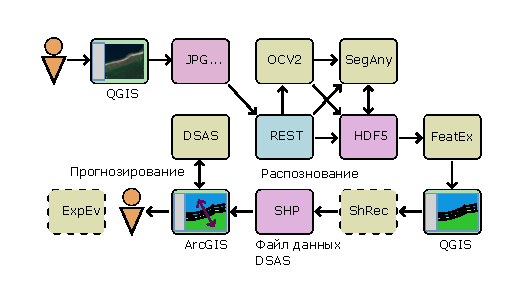
\includegraphics[width=\linewidth]{pics/tech.pdf}
    \caption{Основные процессы в ИВИ поддержки исследований береговых зон водохранилищ}\label{fig:processes}
  \end{figure}
\end{center}

Заметим, что наличие в ИС блоков моделирования и автоматизированной оценки результатов модели формирует базу для создания \emph{систем поддержки принятия решений}, предназначенных для автоматизации выработки \emph{антиинтуитивных решений}.

\subsection{Архитектура системы}
Перечисленные в предыдущем разделе функции и взаимодействия между ними формируют собой элементы архитектуры распределенной системы обработки ГИС-данных (рисунок~\ref{fig:arch}).

\begin{center}
\begin{figure}[htp]
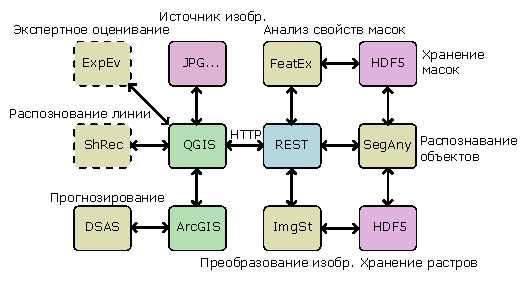
\includegraphics[width=\linewidth]{pics/arch-p.pdf}
  \caption{Архитектура распределенной системы} \label{fig:arch}
\end{figure}
\end{center}

Система состоит из двух основных частей, обычно обозначаемых как <<клиент>> и <<сервер>>. В нашем случае они взаимодействуют друг с другом по протоколу HTTP и реализуют взаимодействие через интерфейс <<архитектуры REST>> (Representation State Protocol). QGIS и ArcGIS - это клиентская часть, она включает также процедуры DSAS, ShRec (распознавание контура), ExpEv (экспертная оценка). QGIS также выступает клиентом для сервера изображений (формат JPG, TIFF, JP2 и др.), получаемых, в том числе, с сервера Google Maps. 

Серверная часть -- набор модулей, запускаемых удаленно из модуля \verb|shore_qgis_module|, т.е. процедурами распознавания управляет полностью   клиентская часть. Управление осуществляется через интерфейс REST, где в качестве объектов выступают сервисы хранения исходных изображений (OCV2 + HDF5), распознавания объектов на изображении (SegAny), анализ масок и изображений с целью получения дополнительных характеристик (FeatEx), сервис выгрузки данных с представлением в JSON (внутри REST). Приведем пример реализации интерфейсов REST для загрузки изображений и управления процессом распознавания.

\subsection{Интерфейс REST загрузки и обработки изображений}
Задача данного программного объекта - принимать бинарный файл изображения, преобразовать его в матрицы слоев, записать в базу данных на сервере, выдать глобальный идентификатор, при помощи которого далее идентифицируется сохраненные данные изображения.
\begin{minted}{python}
img = Service(name='imgstore',
              path='/sa-1.0/image/{img_name}',
              description="Image collection")

@img.put()
def put_image(request):
    """Принимает бинарные данные картинки,
    возвращает JSON с UUID сохраненного изображения
    """
    name = request.matchdict['img_name']

    imgg, ds = add_image(name, request.body)

    uui = uuidgen()
    uuis = str(uui)
    pth = ds.name
    STORAGE, INGRP, UUIDGRP = storage_begin()
    if name in UUIDGRP:
        ouuis = gs(UUIDGRP[name])
        del UUIDGRP[name]
        del UUIDGRP[ouuis]
    # Отображение UUID <-> имя изображения
    UUIDGRP.create_dataset(name, data=uuis)
    UUIDGRP.create_dataset(uuis, data=name)
    STORAGE, INGRP, UUIDGRP = storage_end()
    return {
        "error": None,
        "ok": True,
        "uuid": uuis,
        "content": pth,
        "name": name,
        "namepath": imgg.name
    }

def add_image(name, content, replace=True):
    ”””Добавление изображения в БД”””
    nparr = np.frombuffer(content, np.uint8)
    image = cv2.imdecode(nparr, cv2.IMREAD_COLOR)
    image = cv2.cvtColor(image, cv2.COLOR_BGR2RGB)
    # Открытие БД
    STORAGE, INGRP, UUIDGRP = storage_begin()
    if name in INGRP:
        del INGRP[name]
    imgg = INGRP.create_group(name)
    ds = imgg.create_dataset('content',
              data=image, compression="lzf")
    log.info("Image '{}' loaded".format(name))
    # Закрытие БД
    STORAGE, INGRP, UUIDGRP = storage_end()
    return (imgg, ds)
\end{minted}
Загрузка изображения делается при помощи запроса PUT с адресом \texttt{https://<адрес сервера>:6543/sa-1.0/image/<имя картинки>}. В тело запроса PUT помещается содержимое изображения. В качестве результата возвращается JSON-ответ, содержащий в поле “uuid” идентификатор сохраненного изображения. Список сохраненных изображений получается запуском запроса GET к этому же адресу без указания имени изображения. Возвращается JSON со списком отображений UUID-<имя файла изображения>. Полученный идентификатор используется для обозначения изображения, подвергающегося процедуре распознавания:

\begin{minted}{python}
sactrl = Service(name='segment-any-control',
                 path='/sa-1.0/sa/{img_uuid}/{cmd}',
                 description="Functions of SA on a image\
                              identified by uuid")
@sactrl.post()
def start_recognition(request):
    # Импорт процедур анализа, выполняющихся в
    #  других процессах
    from ..tasks import (sa_start, 
          ANSWERS, rc_set, rc_get, rc_delete,
          rc_update)

    uuids = request.matchdict['img_uuid']
    cmd = request.matchdict['cmd']
    # cmd = 'start'

    STORAGE, INGRP, UUIDGRP = storage_begin()
    # идентификатор изображения существует?
    isimg = uuids in UUIDGRP
    STORAGE, INGRP, UUIDGRP = storage_end()

    rd = {"error": False, "ok": True, "cmd": cmd}

    if cmd == "flush":
        ANSWERS.flushdb()
        return rd

    if not isimg:
        return {
            "error": "not found",
            "ok": False,
            "uuid": uuids,
            "cmd": cmd,
            "processuuid": None
        }
    # Команда запуска процесса распознавания
    if cmd == "start":
        prevrc = rc_get(uuids)
        if prevrc is not None:
            return {
                "error": "already running",
                "ok": False,
                "uuid": uuids,
                "cmd": cmd,
                "processuuid": prevrc.get("processuuid",
                                           None),
                "ready": prevrc.get("ready", False)
            }
        del prevrc
        rc = {"uuid": uuids, "ready": False}
        rc_set(uuids, rc)
        arc = sa_start.delay(uuids)
        puuid = str(arc.id)

        def _u(r):
            r["processuuid"] = puuid

        rc = rc_update(uuids, _u)
        print(rc_get(uuids))
        puuid = rd["processuuid"] = puuid
    # Команда проверки завершения процесса
    elif cmd == "status":
        rd["ready"] = False

        def _a(v, rr):
            rd["ready"] = v
            rd["result"] = rr.get("result", None)

        rc = rc_get(uuids, "ready", _a)
        if rc is None:
            return {
                "error": "no process",
                "ok": False,
                "uuid": uuids,
                "cmd": cmd,
                "ready": None
            }

        rd["processuuid"] = rc["processuuid"]
    # Команда завершения процесса и удаления его данных
    elif cmd == "finalize":
        rcg = rc_get(uuids)
        if rcg is None:
            return {
                "error": "not running",
                "ok": False,
                "uuid": uuids,
                "cmd": cmd,
                "ready": None
            }
        rc_delete(uuids)
        rd.update({"ready": rcg["ready"], 
                   "processuuid": rcg["processuuid"]})
    # Команда отмены процесса
    elif cmd == "discard":
        rcg = rc_get(uuids)
        if rcg is not None:
            return {
                "error": "still running",
                "description":
                "cannot stop SA, wait its finishing. \
                     Use status command.",
                "ok": False,
                "uuid": uuids,
                "cmd": cmd,
                "ready": None
            }
        STORAGE, INGRP, UUIDGRP = storage_begin()
        name = gs(UUIDGRP[uuids])
        imgg = INGRP[name]
        if "masks" in imgg:
            del imgg["masks"]
            rc = "removed"
        else:
            rc = "no mask"
        STORAGE, INGRP, UUIDGRP = storage_end()
        rd.update({
            "ready": None,
            "processuuid": None,
            "description": rc
        })

    return rd
\end{minted}

Запуск процесса распознавания осуществляется при помощи запроса POST следующего формата - \texttt{http://<адрес сервера>:6543/sa-1.0/sa/<идентификатор изображения>/<команда>}. Командой выступает ключевое слово - одно из четырех:
\begin{description}
  \item[start] -- запуск нового процесса, 
  \item[status] -- запрос состояния распознавания,
  \item[finalize] -- завершение исполнившегося процесса,
  \item[flush] -- отмена процесса.
\end{description}
Требующие большие вычислительные ресурсы процессы выполняются в отдельных процессах сервера или на специализированных серверах, снабженных аппаратной поддержкой вычислений (CUDA и ему подобным). Реализация запуска таких задач реализована при помощи библиотеки celery языка программирования Python.

\subsection{Распознавание контура береговой линии}

\subsection{Анализ структуры объектов изображения}

На данном этапе производится классификация объектов -- необходимо соотнести распознанные объекты к классам <<водная поверхность>> и <<суша>>. Модель SA для каждого распознанного объекта сопоставляет так называемую ключевую точку (рисунок~\ref{fig:objsanalysis}). В режиме распознавания <<всех объектов>> на изображении библиотека сканирует изображения по некоторой сетке. Каждой точкой сетки производится указание (prompt) на объект, который необходимо выделить на изображении. Если указанию соответствует новый объект, то этот объект ассоциируется с точкой. Получается, что координаты ключевой точки идентифицируют объект. 
 
\begin{center}
\begin{figure}
  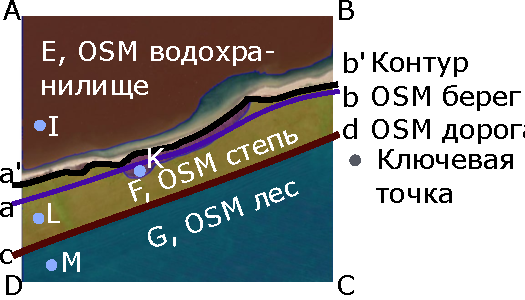
\includegraphics[width=0.7\linewidth]{pics/tracing-p.pdf}  
  \caption{К объяснению идеи распознавания береговой линии при помощи классификации масок SsegmentAnything}\label{fig:objsanalysis}  
\end{figure}
\end{center}

На рисунке~\ref{fig:objsanalysis} точками $I$, $L$, $M$ обозначены объекты $E$, $F$, $G$, соответственно. Для мелкого объекта, соответствующего точке $K$, имя не задано. Точка, таким образом, принадлежит объекту, точнее находится на маске изображения. Чтобы достаточно достоверно определить, является объект водным или сушей, можно выполнить запрос к серверу OpenStreetMap~\cite{OSM} следующего вида:
\begin{minted}{text}
  [out:json];
    (
      is_in(53.5202071,103.3259833); // Координата точки K
    );
    out center;
\end{minted}
В ответ будет получен JSON следующего вида:
\begin{minted}{json}
  {
  "version": 0.6,
  "generator": "Overpass API 0.7.62.1 084b4234",
  "osm3s": {
    "timestamp_osm_base": "2024-06-12T10:11:58Z",
    "timestamp_areas_base": "2024-06-12T05:25:19Z",
    "copyright": "The data included in this document is from www.openstreetmap.org. The data is made available under ODbL."
  },
  "elements": [

{
  "type": "area",
  "id": 3600060189,
  "tags": {
    "ISO3166-1": "RU",
    "ISO3166-1:alpha2": "RU",
    "ISO3166-1:alpha3": "RUS",
    "ISO3166-1:numeric": "643",
    "according_to:RU": "yes",
    "according_to:UA": "no",
    "admin_level": "2",
    "alt_name:eo": "Rusujo;Ruslando",
    "border_type": "nation",
    "boundary": "administrative",
    "currency": "RUB",
    "default_language": "ru",
    "flag": "https://upload.wikimedia.org/wikipedia/commons/f/f3/Flag_of_Russia.svg",
    "int_name": "Russia",
    "int_ref": "RU",
    "name": "Россия",
  // .....
},
// ....
{
  "type": "area",
  "id": 3601221148,
  "tags": {
    "addr:country": "RU",
    "admin_level": "3",
    "boundary": "administrative",
    // .....
}
// ....
\end{minted}
Среди перечисленных объектов нет объекта, обозначающего водный резервуар. Теперь запрос по координате точки I:
\begin{minted}{text}
  [out:json];
    (
      is_in(53.5202071,103.3259833); // Координата точки I
    );
    out center;
\end{minted}
В ответ будет получен JSON следующего вида:
\begin{minted}{json}
// ......
{
  "type": "area",
  "id": 3600167043,
  "tags": {
    "alt_name:cs": "Bratská vodní nádrž",
    "gvr:code": "16010100821416200001042",
    "name": "Братское водохранилище",
    "name:ca": "Embassament de Bratsk",
    "name:cs": "Bratská přehradní nádrž",
    "name:en": "Bratsk Reservoir",
    "name:eo": "Bratska Rezervujo",
    "name:pl": "Zbiornik Bracki",
    "name:ru": "Братское водохранилище",
    "name:sk": "Bratská vodná nádrž",
    "name:zh": "布拉茨克水库",
    "natural": "water",
    "type": "multipolygon",
    "water": "reservoir",   // Тег, определяющий тип водема
    "wikidata": "Q899803",
    "wikipedia": "ru:Братское водохранилище"
  }
},
// ......
\end{minted}
Здесь среди выданных объектов присутствует объект, описанный как водный резервуар. 

Собрав информацию по всем ключевым точкам, теперь становиться возможным объединить все маски, относящиеся к водным объектам, и все маски, относящиеся к суше. Граница суши со стороны водного объекта будет являться приближением береговой линии.

Контур береговой линии из набора пикселей (растра) преобразуется в векторный объект при помощи варианта алгоритма, представленного в \cite{b3}.

Предлагаемый подход также применим к привязанным к координатам аэрофотоснимкам и ортофотопланам.

\chapter{Реализация подсистем распределенной вычислительной среды}\label{chap:impl}


\section{Тестирование}

\chapter*{ЗАКЛЮЧЕНИЕ}

Выпускная квалификационная работа посвящена проекту развития научного направления Лаборатории инженерной геологии и геоэкологии в аспекте повышения уровня информатизации и обработки данных полевых исследований. В работе решены следующие задачи:
\begin{enumerate}
  \item Проведена формализация предметной области инженерной геологии, относящейся к исследованиям экзогенных геологических процессов на берегах крупного внутреннего водоёма, представлена концептуальная модель в виде онтологии,
  \item Разработана информационно-вычислительной инфраструктура поддержки прогнозирования состояния береговой зоны на основе геоинформационной системы и распределенной вычислительной среды,
  \item Предложен вариант архитектуры вычислительной среды,  реализованы некоторые её подсистемы с использованием современных средств автоматизации распознавания объектов на изображениях,
  \item Для реализованных подсистем предложены модели данных, предназначенных для хранения информации в процессе её обработки,
  \item Продемонстрирована работоспособность предложенной среды на простом примере прогнозирования.
\end{enumerate}

Рассмотренные в диссертации вопросы преследуют целью формирование вычислительных ресурсов поддержки принятия решений по результатам мониторинга, оценки и прогноза опасных геологических процессов. Дальнейшее направление научных исследований и опытно-конструкторских работ имеет смысл продложать по нескольким основным направлениям:
\begin{itemize}
  \item Завершение реализации информационно-вычислительный среды,
  \item Наполнение информационных ресурсов архивными данными и данными современного мониторинга объектов исследования,
  \item Совершенствование методов прогнозирования состояния береговой зоны за счет реализации современного уровня информационного обеспечения,
  \item Разработка экспертной системы оценки результатов моделирования с целью формирования рекомендаций по использованию конкретных участков исследуемой береговой зоны.
\end{itemize}

Преимущества рассмотренного подхода -- это а) отсутствие трудоемкого этапа подготовки данных для обучения НС, б) распознавание контура представляется (программируется) в виде правил, что дает возможность управлять процессом распознавания, в частности “сцеплять” объекты или контуры с разных изображений; в) SA, ввиду обученности на большом количестве изображений не привязана к свойствам конкретных изображений (размеру, цветовой гамме, повороту и т.д.), что позволяет г) реализовывать (в перспективе) процедуры последовательного уточнения характеристик береговой линии, переходя к изображениям более высокого разрешения.

Разработанная платформа и модели обеспечат более эффективный способ оцифровки данных с изображений, результаты будут востребованы во многих проектных, изыскательских и научно-исследовательских организациях для проведения комплексных оценок, прогнозирования и принятия решений по управлению различными объектами береговой зоной для обеспечения их безопасного и рационального использования.
     

\begin{thebibliography}{99}


  \bibitem{gruber} Thomas R. Gruber,
Toward principles for the design of ontologies used for knowledge sharing?,
International Journal of Human-Computer Studies,
Vol. 43, No. 5–6,
1995,
Pp. 907-928,
ISSN 1071-5819,
\doi{10.1006/ijhc.1995.1081}, \url{https://www.sciencedirect.com/science/article/pii/S1071581985710816} (дата доступа: 11.05.2024)

\bibitem{b1} Dang K. B., Vu K. C., Nguyen H., Nguyen D. A., \emph{et al.}. Application of deep learning models to detect coastlines and shorelines. // Journal of Environmental Management, 2022, No.~320, 115732.

\bibitem{b2} Seale C., Redfern T., Chatfield P., Luo C., Dempsey K. Coastline detection in satellite imagery: A deep learning approach on new benchmark data // Remote Sensing of Environment, 2022, No.~278, 113044.

\bibitem{b3} Aghdami-Nia M., Shah-Hosseini R., Rostami A., Homayouni S. Automatic coastline extraction through enhanced sea-land segmentation by modifying Standard U-Net // International Journal of Applied Earth Observation and Geoinformation, 2022, No.~109, 102785.

\end{thebibliography}




\end{document}
